\documentclass[unicode,11pt]{beamer}
\usepackage{luatexja}
\usepackage[ipaex]{luatexja-preset}
\usepackage{amsmath}
\usepackage{array}
\renewcommand{\kanjifamilydefault}{\gtdefault}


\usetheme{Madrid}

\title{中間発表}
\subtitle{最適配置問題へのPrincipal Pointsの応用}
\author{計数工学科 数理情報工学コース4年\\梶山拳太郎}
\date{\today}
\institute{指導教員:松田孟留准教授}

\begin{document}

\begin{frame}
    \titlepage
\end{frame}

\begin{frame}{施設配置問題}
    \begin{itemize}
        \item 与えられた人口分布をもとに最適な施設配置に関する問題を考えたい。
        \item 施設配置コストは利用者と施設の距離に比例すると考えられる.
    \end{itemize}
    \begin{figure}[htbp]
        \begin{minipage}[b]{0.48\linewidth}
            \centering
            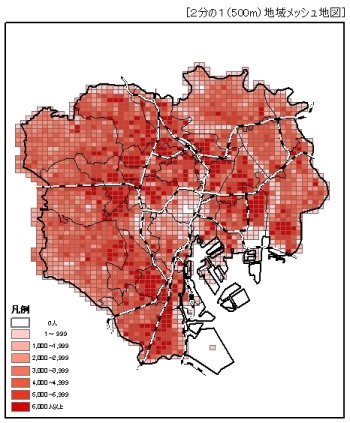
\includegraphics[keepaspectratio, scale=0.4]{tokyo_mesh_h22.jpeg}
            \caption{地域メッシュ統計(総務省統計局:「平成22年国勢調査に関する地域メッシュ統計」より引用)}
        \end{minipage}
        \begin{minipage}[b]{0.48\linewidth}
            \centering
            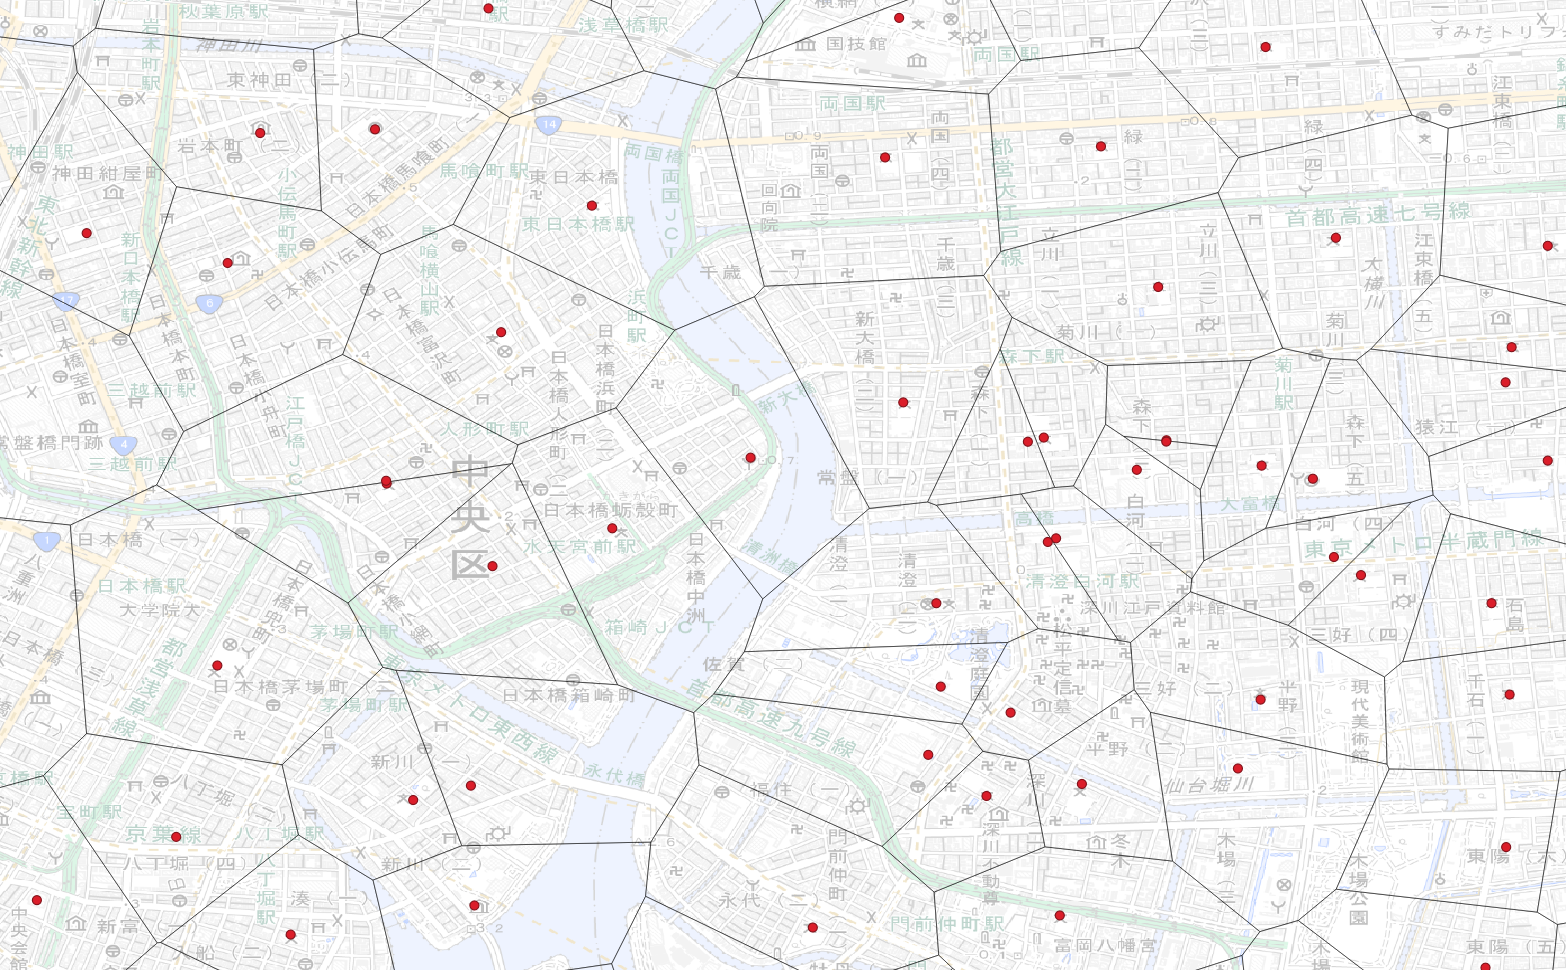
\includegraphics[keepaspectratio, scale=0.1]{Tokyo_Chuoku_Voronoi_2.png}
            \caption{地図上のボロノイ図}
        \end{minipage}
    \end{figure}
\end{frame}

\begin{frame}{Principal Points}
    \begin{itemize}
        \item k個の点の最適配置を考えるため,k-Principal Pointsを導入する.
    \end{itemize}
    \begin{block}{距離の定義}
        $y_j \in R^p (1\le j \le k)$はp次元ユークリッド空間のk個の点.$x \in  R^p$と$k$個の点$y_j (1 \le j \le k)$との距離は,
        \begin{equation*}
            d(x|y_1,\dots,y_k) = \min_{1\le j \le k}{\{(x-y_j)^{\mathrm{T}}(x-y_j)\}}^{\frac{1}{2}}
        \end{equation*}
    \end{block}
    \begin{block}{k-Principal Pointsの定義}
        $X$は$R^p$内の確率変数,$E$は$X$についての期待値.
        \begin{equation*}
            v_1,v_2,\dots,v_k = \underset{y_j \in R^p, 1\le j \le k}{\operatorname{argmin}} E\{d^2(X|y_1,\dots, y_k)\}
        \end{equation*}
    \end{block}
\end{frame}

\begin{frame}{Principal Points}
    \begin{itemize}
        \item Principal Pointsは[Flury,1990]より提案された.
        \item 与えられた確率分布の密度関数をk個の領域に分割する際の各領域の中心点と考えられる.
    \end{itemize}
    \begin{figure}
        \centering
        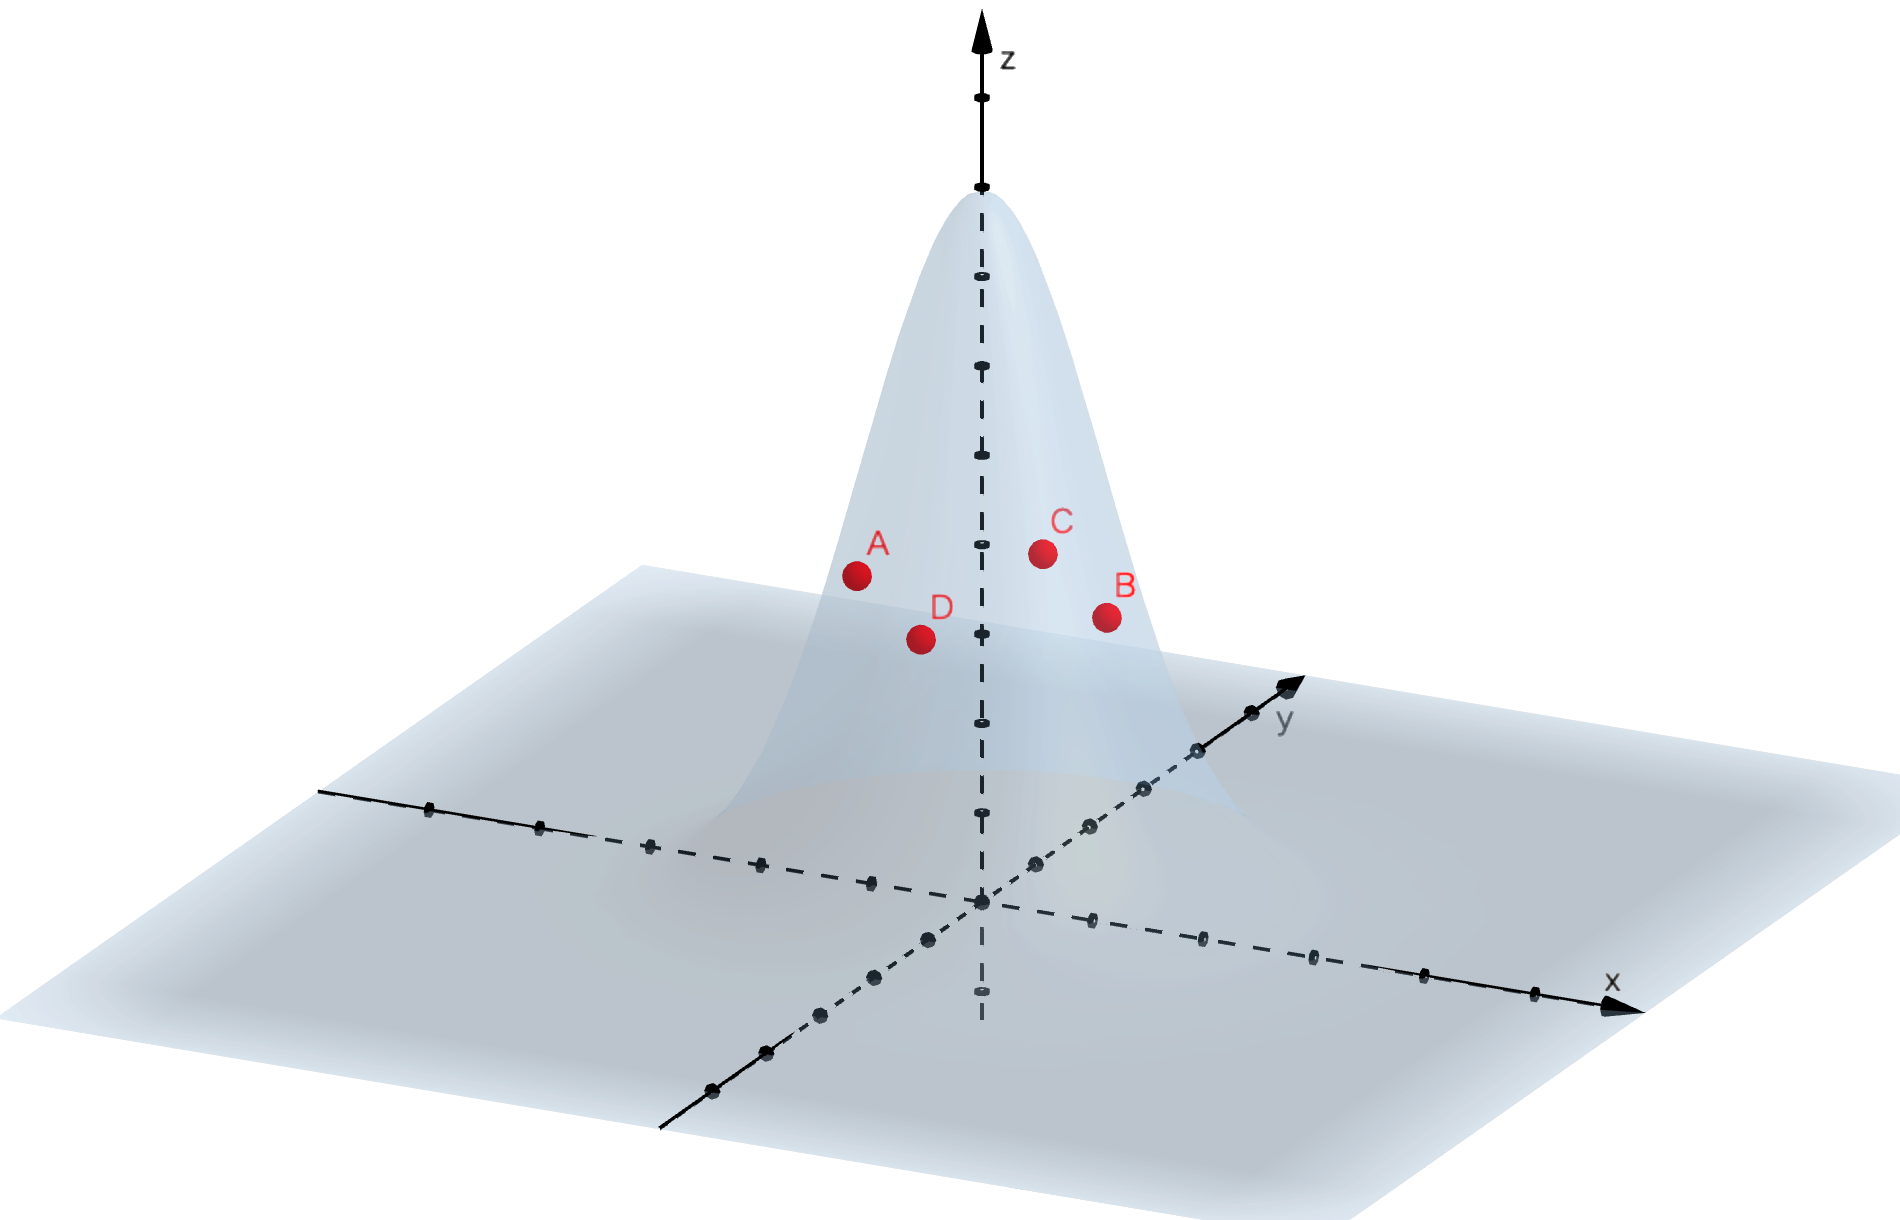
\includegraphics[keepaspectratio,scale = 0.2]{4-principal_points.png}
        \caption{例:4-Principal Points}
    \end{figure}
\end{frame}

\begin{frame}{研究の方針}
    \begin{itemize}
        \item $L_2$ノルムの2乗の期待値最小化を定義としたPrincipal Pointsの性質、応用に関する研究が多い.
        \item 本研究では$L_2$ノルムの1乗の期待値最小化を定義としたPrincipal Pointsの性質,応用を中心に考える.
        \item 既存手法とノルムの1乗での方法による人口分布実データを利用した最適配置問題を考える.
    \end{itemize}
\end{frame}

\begin{frame}{ノルムの2乗と1乗}
    \begin{block}{k-Principal Points(再掲)}
        \begin{equation*}
            v_1,v_2,\dots,v_k = \underset{y_j \in R^p, 1\le j \le k}{\operatorname{argmin}} E\{d^2(X|y_1,\dots, y_k)\}
        \end{equation*}
    \end{block}

    \begin{block}{k-Principal Points(1乗の場合)}
        \begin{equation*}
            v_1,v_2,\dots,v_k = \underset{y_j \in R^p, 1\le j \le k}{\operatorname{argmin}} E\{d^1(X|y_1,\dots, y_k)\}
        \end{equation*}
        ただし,
        \begin{equation*}
            d^1(x|y_1,\dots,y_k) = \min_{1\le j \le k}{\lVert x_j - y_j\rVert_2^1}
        \end{equation*}
    \end{block}
    2乗の場合はデータの平均値として導出されるが,1乗の場合にはデータの中央値を考えることになる.(Geometric Median)
\end{frame}

\begin{frame}{Geometric medianについて}
    \begin{columns}
        \begin{column}{0.48\textwidth}
            \begin{itemize}
                \item 1乗の場合の代表点はGeometric Medianと呼ばれる.
                \item 右図は[Vardi \& Zhang,2000]のアルゴリズムによる計算例.
            \end{itemize}
        \end{column}
        \begin{column}{0.48\textwidth}
            \begin{figure}
                \centering
                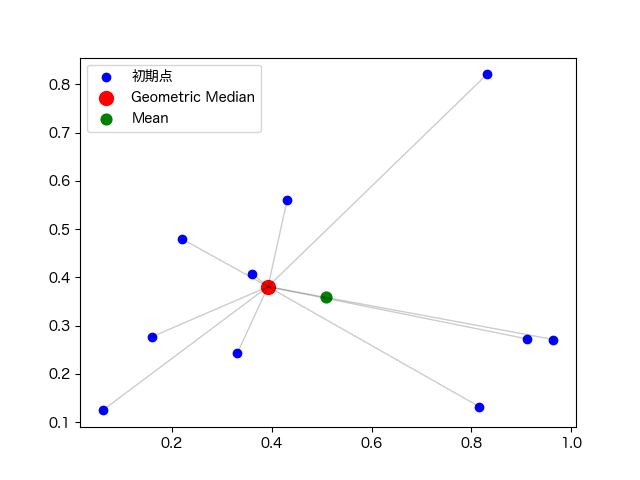
\includegraphics[keepaspectratio, scale = 0.35]{Geometric_Median.png}
                \caption{Geometric Median}
                \label{Geometric_Median}
            \end{figure}
        \end{column}
    \end{columns}
\end{frame}

\begin{frame}{$d^1$と$d^2$の比較}
    \begin{table}[ht]
        \centering
        \begin{tabular}{|c|c|c|}
            \hline
            要約点の個数\textbackslash 距離の取り方& \textbf{$d^1$} & \textbf{$d^2$} \\
            \hline
            \textbf{1点のみ} & Geometric Median & Mean \\
            \hline
            \textbf{k点} & 本研究 & k-means \\
            \hline
        \end{tabular}
        \caption{$d^1$と$d^2$の比較}
        \label{tab:comparison}
    \end{table}
    \begin{figure}[htbp]
        \begin{minipage}[b]{0.48\linewidth}
            \centering
            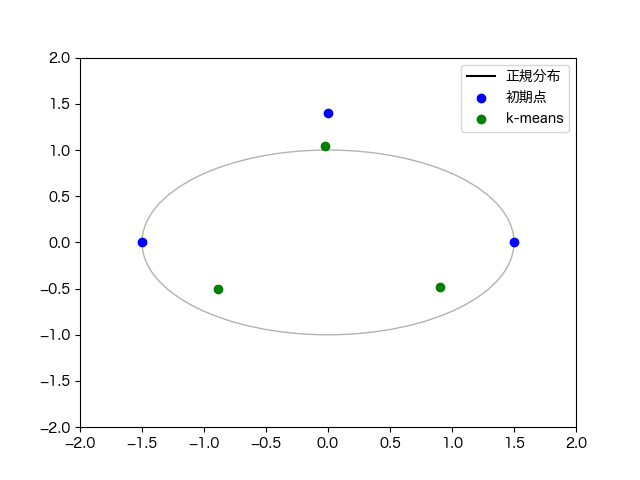
\includegraphics[keepaspectratio, scale=0.30]{Nontitlek-meansonly.png}
            \caption{k-means法による3-Principal Points}
        \end{minipage}
        \begin{minipage}[b]{0.45\linewidth}
            \centering
            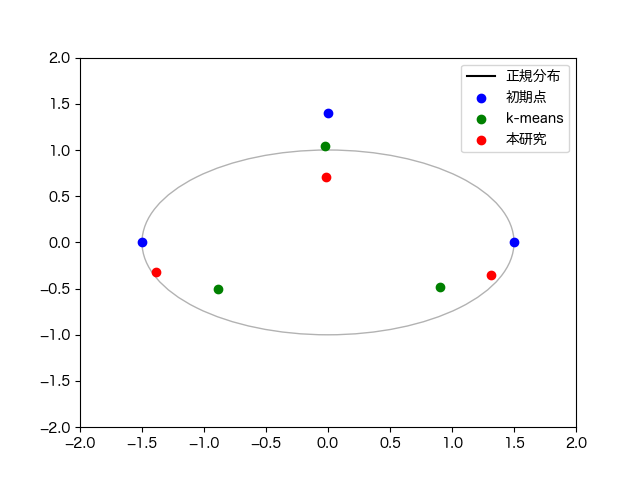
\includegraphics[keepaspectratio, scale=0.30]{Nontitlek-meansandmedian.png}
            \caption{k-means法及び本研究による3-Principal Points}
        \end{minipage}
    \end{figure}
\end{frame}

\begin{frame}{今後の研究について(1):$d^1$と$d^2$の応用時の比較}
    \begin{itemize}
        \item コスト関数が距離に比例すると仮定して1乗の場合の公共施設等の最適配置問題を考える.
        \item 1乗の場合と2乗の場合の結果を比較する際の評価基準を定めることが今後の課題.
    \end{itemize}
\end{frame}
\begin{frame}{今後の研究について(2):実データへの応用}
    \begin{itemize}
        \item [栗田,2004,2013]では東京の人口分布及びそれに伴う交通網は中心点(例,皇居)を基準に放射状に伸びていると考え,2次元→1次元の近似を行なって施設配置を考えている.
        \item このような1次元モデルによる結果と2次元データから考えた場合の配置とを比較,考察する.
    \end{itemize}
    \begin{figure}[htbp]
        \begin{minipage}[b]{0.45\linewidth}
            \centering
            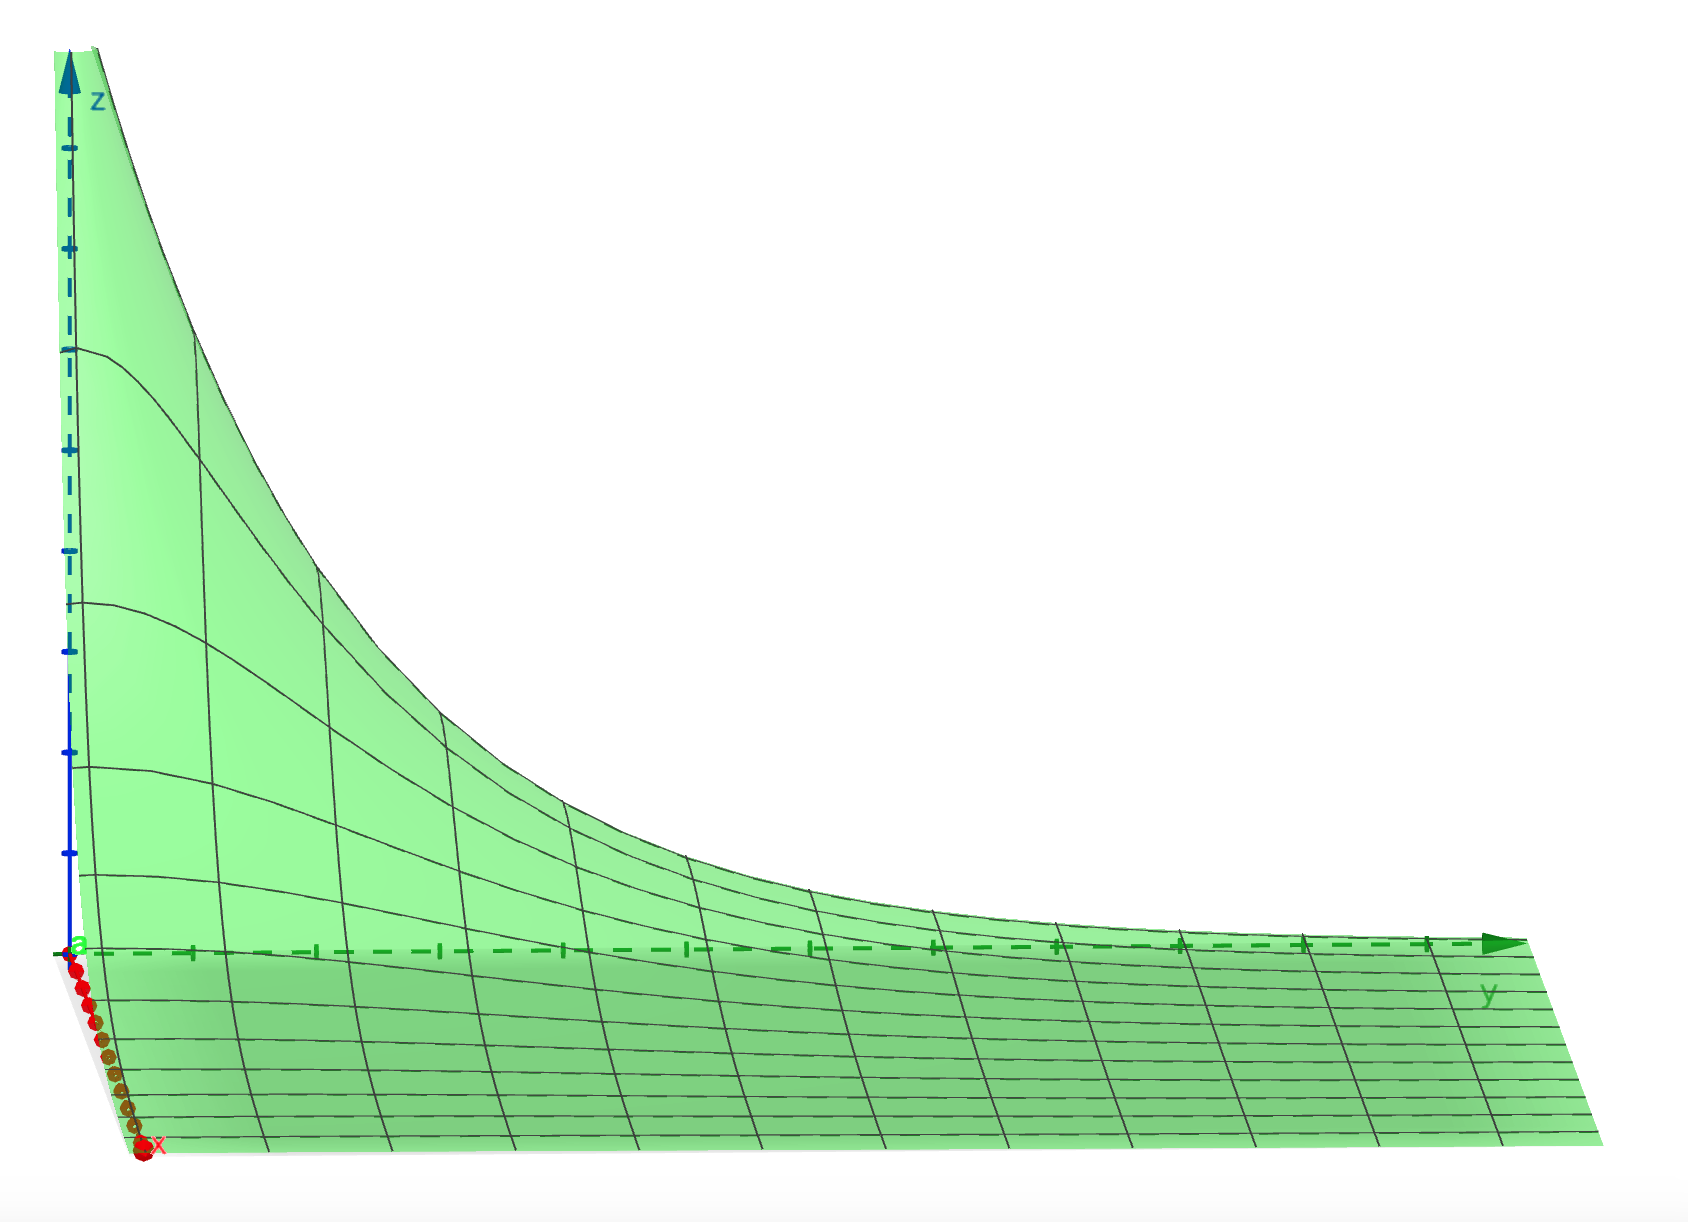
\includegraphics[keepaspectratio, scale=0.15]{z=e-u.png}
            \caption{回転対称な人口分布モデル}
        \end{minipage}
        \begin{minipage}[b]{0.45\linewidth}
            \centering
            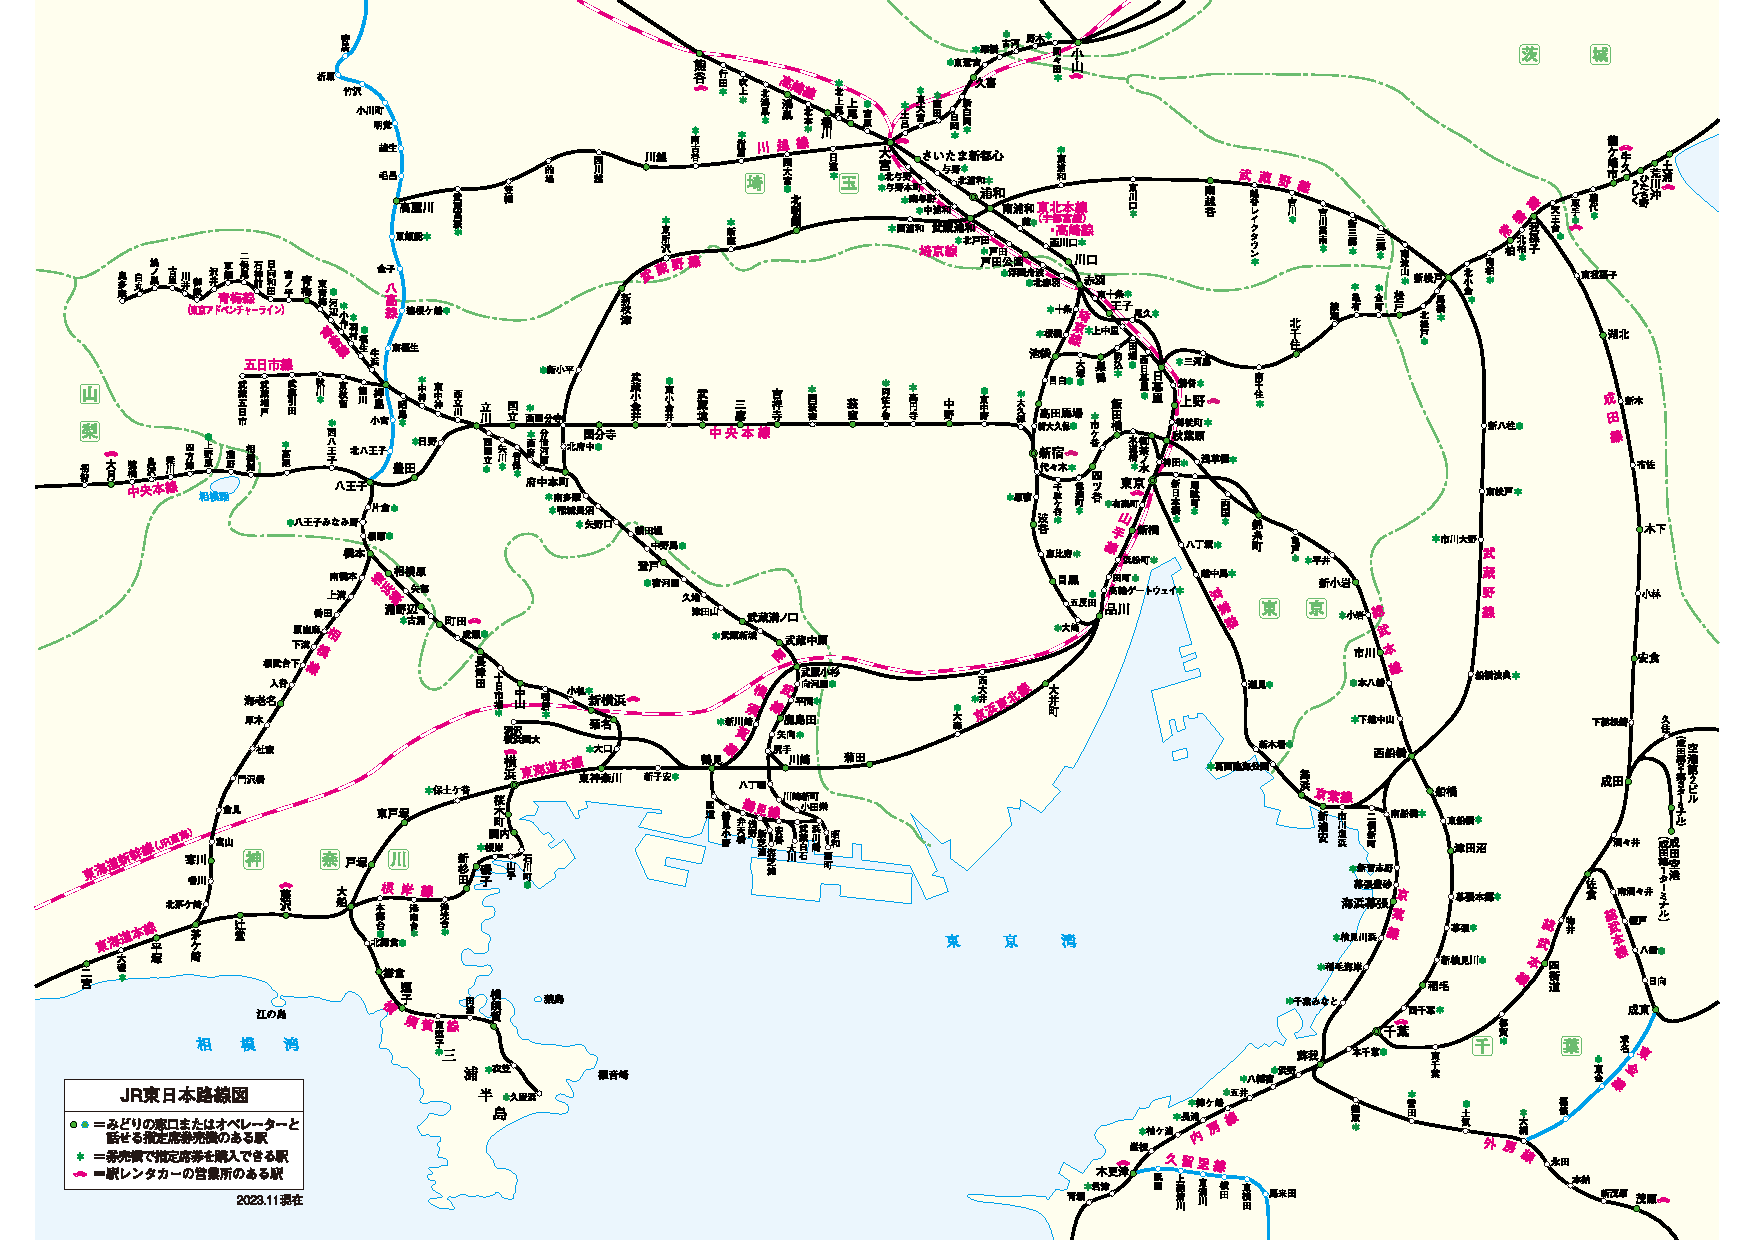
\includegraphics[keepaspectratio, scale=0.15]{tokyo.pdf}
            \caption{関東路線図(JR東日本:「路線図,東京近郊エリア」より引用}
        \end{minipage}
    \end{figure}
\end{frame}

\begin{frame}{参考文献}
    \begin{thebibliography}{99}
        \bibitem{Flury1990}Flury,B. Principal points. Biometrika. 1990, 77, 1, pp. 33-41.
        \bibitem{Flury1993}Flury,B. Estimation of Principal points. Journal of the Royal  Statistical Society. 1993, 42, 1, pp. 139-151.
        \bibitem{Median_algorithm}Vardi,Y. \& Zhang, C-H. The multivariate $L_1$-median and associated data depth. Proceedings of the National Academy of Sciences of the United States of America. 2000, 97, 4, pp. 1423-1426.
        \bibitem{Shimizu}清水信夫,水田正弘,佐藤義治. Principal points の性質について. 応用統計学. 1998, 27, 1.
        \bibitem{Okabe}岡部篤行,鈴木敦夫 (1992). 最適配置の数理 ーシリーズ現代人の数理3ー. 朝倉書店
        \bibitem{Kuritabook1}栗田治 (2013). 都市と地域の数理モデル. 共立出版.
        \bibitem{Kuritabook2}栗田治 (2004). 都市モデル読本. 共立出版.
    \end{thebibliography}
\end{frame}

\begin{frame}{参考文献}
    \begin{thebibliography}{99}
        \bibitem{Mesh}総務省統計局. ”平成22年国勢調査に関する地域メッシュ統計”. 総務省統計局. https://www.stat.go.jp/data/mesh/h22\_w.htm,(参照 2023-12-4).
        \bibitem{JR}JR東日本. "路線図". JR東日本. https://www.jreast.co.jp/map/pdf/tokyo.pdf, (参照 2023-12-4).
    \end{thebibliography}
\end{frame}

\end{document}